



\section{Test Automata}
Several automata generated randomly using different parameters were used in the testing process. Three major different techniques of generation were used:

\begin{enumerate}
	\item Use Spot (\cite{}) to generate a random DPA. (called \emph{gendet})
	\item Use Spot to generate a random non-deterministic B\"uchi automaton and use Spot again to convert it to a DPA. (called \emph{detspot})
	\item Use Spot to generate a random non-deterministic B\"uchi automaton and use nbautils (\cite{}) to convert it to a DPA. (called \emph{detnbaut})
\end{enumerate}

Figures \ref{exp:fig:rawstats_size}, \ref{exp:fig:rawstats_prios}, \ref{exp:fig:rawstats_sccs}, and \ref{exp:fig:rawstats_langclas} present some information about the automata. Regarding the number of states we stopped the generation at about 100 states, as most algorithms become too slow at that point. For the detnbaut set, the path refinement procedure can be sped up which is why the upper limit is higher. We elaborate this point in the relevant section.

The number of priorities is rather small in general. For gendet, we intentionally limited the number to 4 to mimic real world behavior that can be found in the detnbautils set. In comparison to nbautils, Spot does not perform priority reduction on the determinization result which explains why the detspot automata use more priorities in general.

The number of SCCs is consistently small among all three sets. detspot and gendet contain a few examples of automata with up to 60 SCCs but these are extreme outliers. This low number of SCCs is important to consider, as multiple of the algorithms such as the skip merger perform better the less connected the automaton is.

Finally, the average size of equivalence classes $\mathfrak{C}(\equiv_L)$. Again, this is of relevance to some of the reduction algorithms such as LSF as only states which are language equivalent can be merged. We can observe that the gendet set almost entirely consists of trivial classes (i.e. classes of size 1) while detspot and detnbaut show more promise in that regard.


\begin{figure}
	\centering
	\begin{minipage}{0.49\textwidth}
		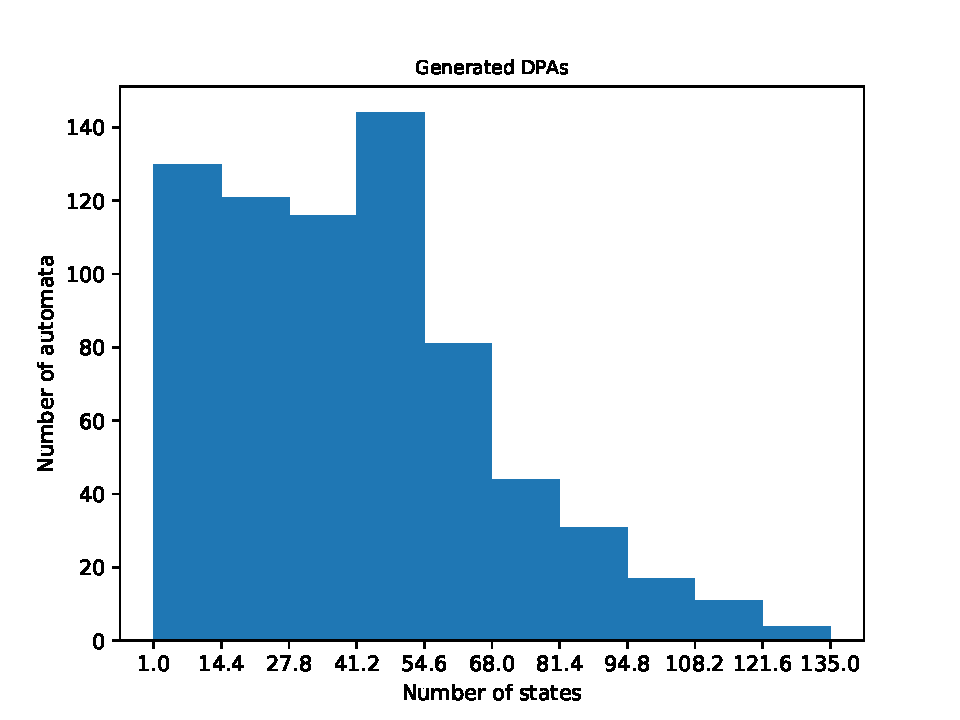
\includegraphics[page=1,height=.3\textheight]{../data/analysis/rawstats_gendet.pdf} 
		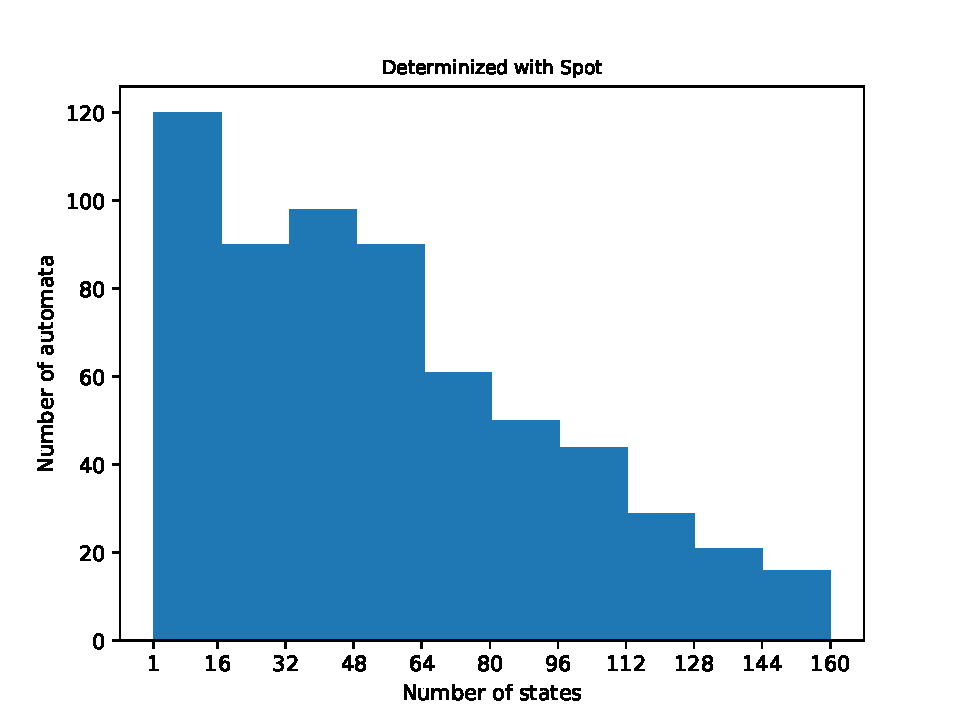
\includegraphics[page=1,height=.3\textheight]{../data/analysis/rawstats_detspot.pdf} 
		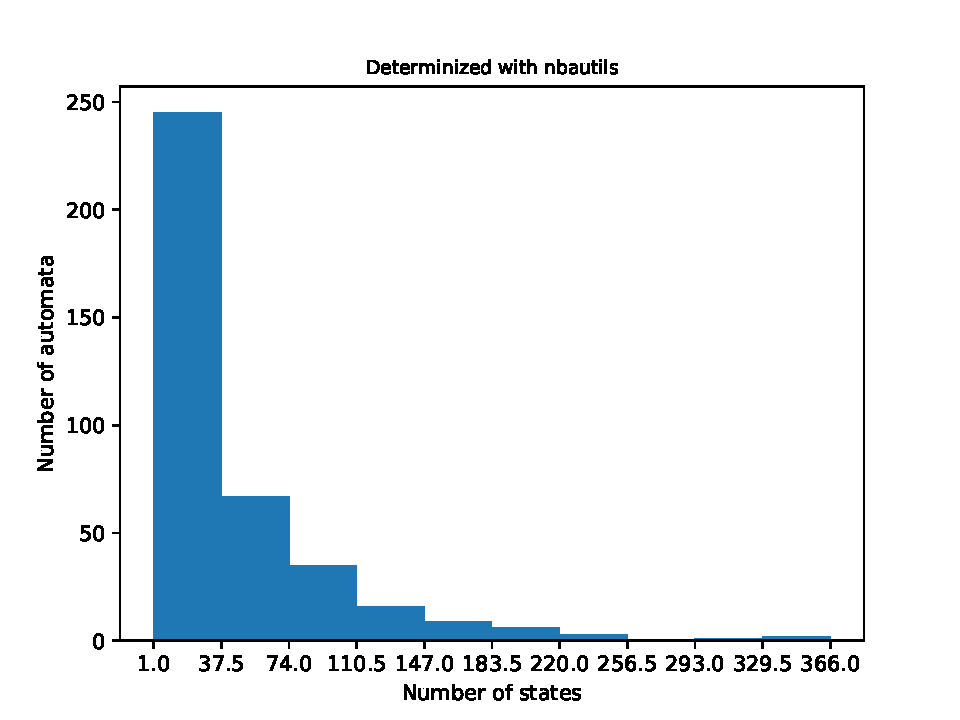
\includegraphics[page=1,height=.3\textheight]{../data/analysis/rawstats_detnbaut.pdf}
		\caption{Sizes of the automata in the testing environment.}
		\label{exp:fig:rawstats_size}
	\end{minipage}
	\hfill
	\begin{minipage}{0.49\textwidth}
		\includegraphics[page=2,height=.3\textheight]{../data/analysis/rawstats_gendet.pdf} 
		\includegraphics[page=2,height=.3\textheight]{../data/analysis/rawstats_detspot.pdf} 
		\includegraphics[page=2,height=.3\textheight]{../data/analysis/rawstats_detnbaut.pdf}
		\caption{Number of priorities in the automata in the testing environment.}
		\label{exp:fig:rawstats_prios}
	\end{minipage}
\end{figure}

\begin{figure}
	\centering
	\begin{minipage}{0.49\textwidth}
		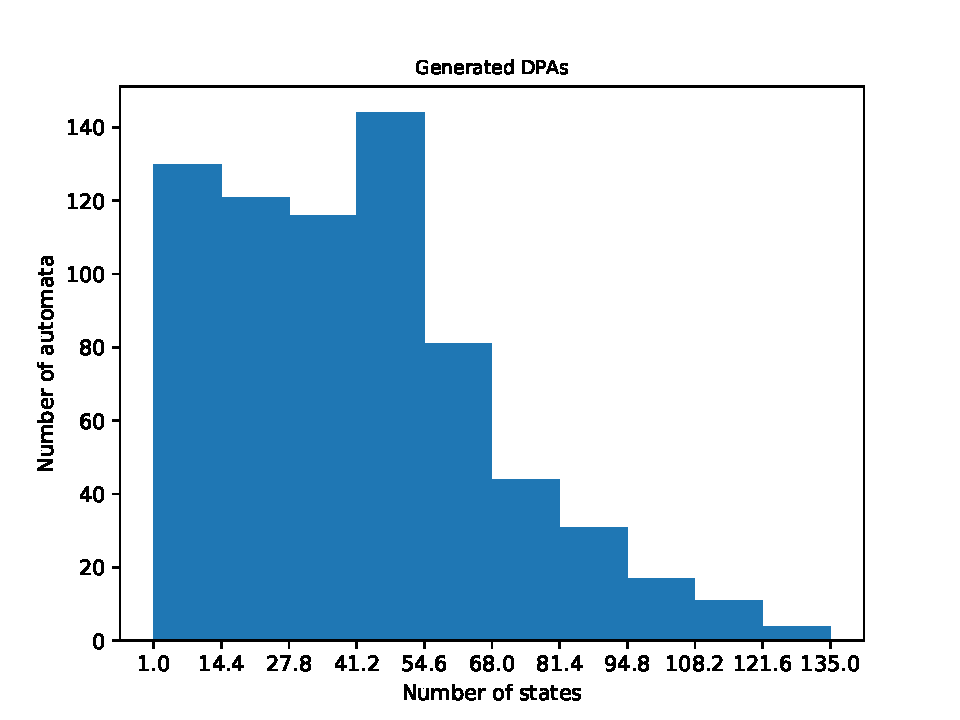
\includegraphics[page=1,height=.3\textheight]{../data/analysis/rawstats_gendet.pdf} 
		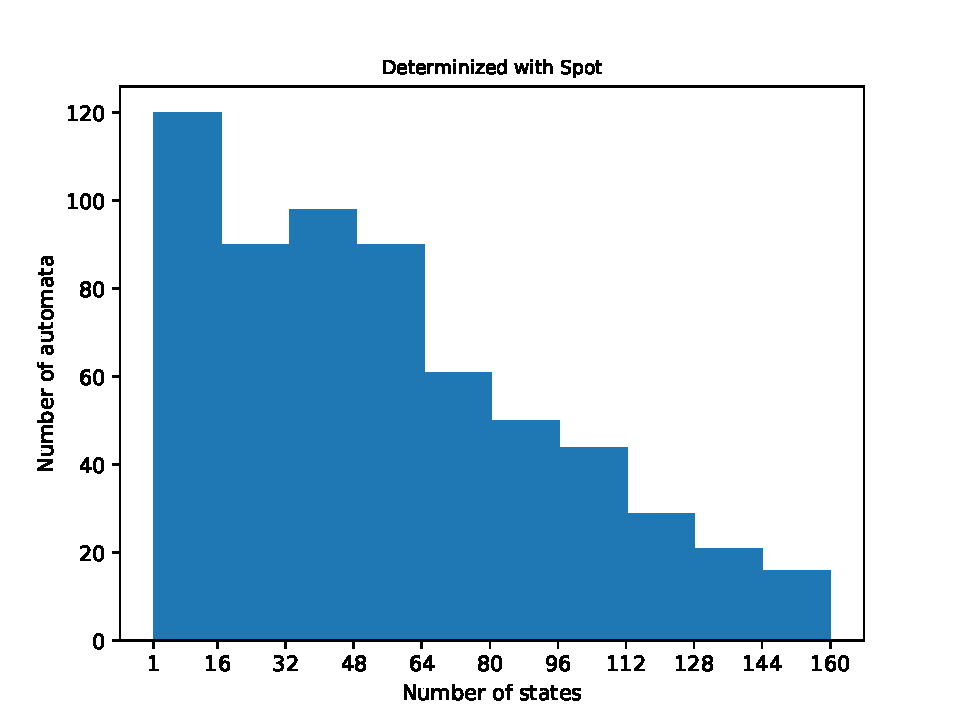
\includegraphics[page=1,height=.3\textheight]{../data/analysis/rawstats_detspot.pdf} 
		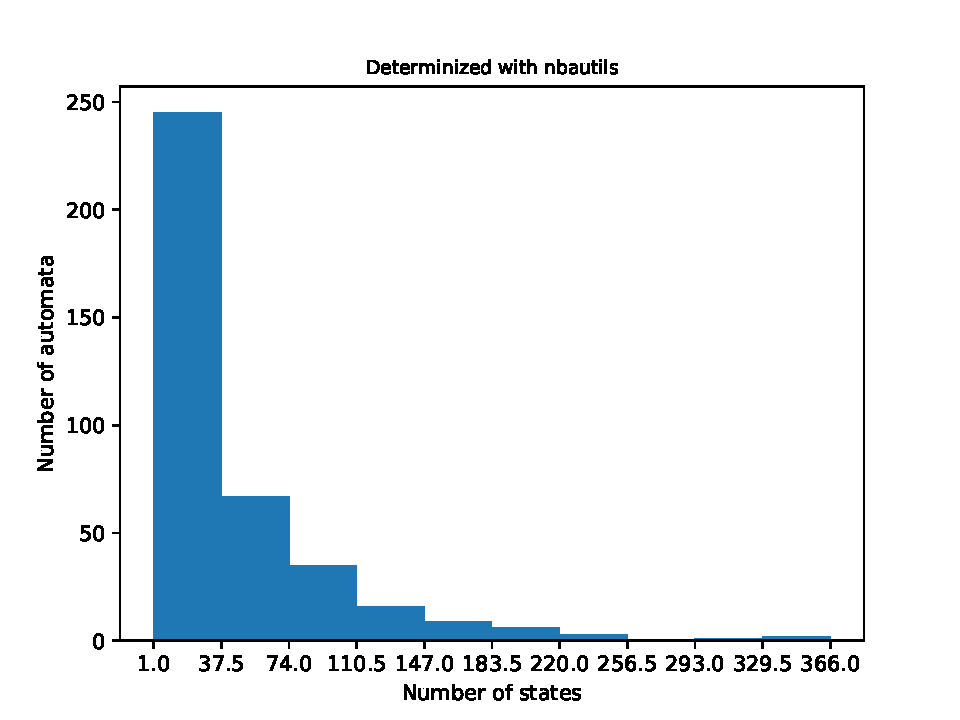
\includegraphics[page=1,height=.3\textheight]{../data/analysis/rawstats_detnbaut.pdf}
		\caption{Number of SCCS in the automata in the testing environment.}
		\label{exp:fig:rawstats_sccs}
	\end{minipage}
	\hfill
	\begin{minipage}{0.49\textwidth}
		\includegraphics[page=2,height=.3\textheight]{../data/analysis/rawstats_gendet.pdf} 
		\includegraphics[page=2,height=.3\textheight]{../data/analysis/rawstats_detspot.pdf} 
		\includegraphics[page=2,height=.3\textheight]{../data/analysis/rawstats_detnbaut.pdf}
		\caption{Average size of $\equiv_L$-classes of the automata in the testing environment.}
		\label{exp:fig:rawstats_langclas}
	\end{minipage}
\end{figure}


